\documentclass[12pt]{article}
\usepackage{xeCJK}

\usepackage{charter}
\usepackage{fullpage}
\usepackage[colorlinks=false]{hyperref}
\usepackage{ifthen}
\usepackage{comment}
\usepackage[title,titletoc]{appendix}
\usepackage{pagecolor}
\usepackage{amsmath}
\usepackage{amsfonts}
%\usepackage[normalem]{ulem}
\usepackage{siunitx}
\usepackage{amsthm}
\sisetup{per=slash, load=abbr}
\usepackage{paralist}
\usepackage{pgfplots}
\usetikzlibrary{positioning}
\usetikzlibrary{fit}
\usetikzlibrary{snakes}
\usetikzlibrary{shapes.geometric}
\usetikzlibrary{patterns}
\usetikzlibrary{shapes,arrows,chains}
\usepgfplotslibrary{patchplots,colormaps}
\usetikzlibrary{calc}
\usetikzlibrary{positioning, fit}
\usetikzlibrary{backgrounds}
\usetikzlibrary{intersections}

\newcommand{\whitepaper}[1]{\begin{center}\fbox{\parbox{0.75\textwidth}{{\small
#1}}}\end{center}}

\newcommand{\pcolor}{violet!25}

\usepackage{setspace}
\usepackage{algorithm2e}
\bibliographystyle{ieeetr}

\usepackage{geometry}
\geometry{left=3cm,right=3cm,top=1.6cm,bottom=3cm,headheight=0pt,headsep=1.5em}
\usepackage{fancyhdr}
\pagestyle{fancy}
\chead{
\includegraphics[scale=0.2]{../common/Nebulas.png}}  %在此处插入logo.pdf图片 图片靠左
\lhead{} % 页眉中间位置内容
\rhead{}
\usepackage{expl3}
\ExplSyntaxOn
\newcommand\latinabbrev[1]{
  \peek_meaning:NTF . {% Same as \@ifnextchar
    #1\@}%
  { \peek_catcode:NTF a {% Check whether next char has same catcode as \'a, i.e., is a letter
      #1.\@ }%
    {#1.\@}}}
\ExplSyntaxOff

%Omit final dot from each def.
\def\eg{\latinabbrev{e.g}}
\def\etal{\latinabbrev{et al}}
\def\etc{\latinabbrev{etc}}
\def\ie{\latinabbrev{i.e}}
\newcommand{\dapp}{DApp\xspace}

%\setlength{\topskip}{1em}

\usepackage{indentfirst}


\setCJKmainfont[BoldFont = STSongti-SC-Bold]{STSongti-SC-Regular}
\setCJKfamilyfont{hei}{SIL-Hei-Med-Jian}		%宋体
\setCJKfamilyfont{song}{SimSun}		%宋体
\setCJKfamilyfont{kai}{Kaiti}		%楷体
\setCJKfamilyfont{fang}{song}	%仿宋
\setCJKfamilyfont{li}{song}			%隶书
\setCJKfamilyfont{you}{Yuanti}		%幼圆

\newcommand{\song}{\CJKfamily{song}}	%宋体
\newcommand{\hei}{\CJKfamily{hei}}	%黑体
\newcommand{\kai}{\CJKfamily{kai}}	%楷体
\newcommand{\fs}{\CJKfamily{fang}}	%仿宋
\newcommand{\li}{\CJKfamily{li}}		%隶书
\newcommand{\you}{\CJKfamily{you}}	%幼圆
\newcommand{\reffig}[1]{图\ref{#1}}
\newcommand{\refsec}[1]{\S \ref{#1}}

\onehalfspacing   % ----------设置1.5倍行距(可能有意义,待调整)

%\parindent=20pt  % -------------------首行缩进大小,英文分段就直接0pt了吧。
\setlength{\parindent}{2.1em}
\setlength{\parskip}{0.3\baselineskip}
\newcommand{\nrcore}{Core Nebulas Rank}
\newcommand{\nrext}{Extended Nebulas Ranks}
\newcommand{\dom}{{\; \texttt{dom}\;}}

\setCJKsansfont[BoldFont = STHeitiSC-Medium]{STHeitiSC-Light}


\newtheorem{property}{特征}
%\addbibresource{reference.bib}

\begin{document}
\pagestyle{empty}
\renewcommand{\contentsname}{目录}
\renewcommand{\abstractname}{摘要}
\renewcommand{\refname}{参考文献}
%\renewcommand{\nomname}{术语表(按首字母排序)}
\renewcommand{\figurename}{图}
\renewcommand{\tablename}{表}
\renewcommand{\baselinestretch}{1.5}
\renewcommand{\appendixname}{附录}
\renewcommand{\proofname}{证明}

\pagecolor{\pcolor}

\begin{titlepage}
  \begin{center}
    \vspace*{5.5cm}
    
\includegraphics[scale=0.5]{../common/Nebulas.png}
    \vspace{0.5cm}


    \textbf{\huge{星云指数黄皮书}}

    \vspace{0.5cm}
    星云研究院
    \vfill
    2018年6月 \\
    版本号:1.0.1
    \textbf{}
  \end{center}

\end{titlepage}
\setcounter{page}{0}
%\thispagestyle{empty}
\tableofcontents
\newpage
\setcounter{page}{1}
\pagestyle{fancy}
\vspace*{0.01cm}
\section{Introduction}

Generally, developers develop applications on some application platforms (like
Windows\footnote{\url{https://www.microsoft.com/en-us/windows}}, Linux\footnote{\url{https://en.wikipedia.org/wiki/Linux}},
macOS\footnote{\url{https://en.wikipedia.org/wiki/MacOS}},
iOS\footnote{\url{https://en.wikipedia.org/wiki/IOS}},
Android\footnote{\url{https://en.wikipedia.org/wiki/Android}} \etc) and
benefit from their applications in traditional software development industry.
The way to get the benefits varies for different developers, including but not
limited to salaries paid by software enterprises, revenue by selling the
application licenses or displaying advertises in their applications.

However, the enterprises who build the application platforms also benefit
from the applications, while the benefits are not shared with the developers.
Let's take the operating system as an example here: a UI/UX designer wants to use \texttt{Sketch},
as we know that the application only works on \texttt{macOS} device, so besides
paying for the application itself, the designer needs to pay Apple\footnote{\url{https://en.wikipedia.org/wiki/Apple_Inc.}}
for the device  to use the application. Apparently, Apple benefits from such user while
Apple does not share the benefits with the \texttt{Sketch} developers.
Another similar example is that users have to pay Apple or
Microsoft\footnote{\url{https://en.wikipedia.org/wiki/Microsoft}} to use
AutoCAD\footnote{\url{https://en.wikipedia.org/wiki/AutoCAD}}. In such cases,
the key factor that users choose a platform is whether the platform
supports required applications for users. In other words, high-quality
applications are critical to the development of an application platform. Based on the above considerations,  application platforms ignore the interests of developers, to a certain extent, infringing the interests of developers.

In the blockchain industry, the interests of \dapp(Decentralized Application) developers are ignored by platforms  as  well.
 In 2004, Ethereum community proposed ``Smart Contract'',
which extended blockchains' ability from peer-to-peer
cryptocurrency networks to decentralized application platforms. However, in comparison with traditional centralized development industry, the ways of obtaining revenue for developers have no significant difference --- decentralized application developers still can not benefit
 from the increment of the blockchain system's value.


Generally speaking,  new-block rewards represent incremental values of the blockchain system and the distribution of such rewards determines the incentive direction of the decentralize system. In our opinion, a blockchain system's incremental value essentially comes from the implicit values from users' data, which should be distributed to all contributed parties, including \dapp deveploers. However, what we see in practice is that, in most PoW blockchain systems, represented by Bitcoin, new-block rewards are distributed to miner nodes; In PoS (proof of stake) based blockchain systems, new-blocks rewards are assigned to  stake holders. Along with it, the interests of \dapp developers are somewhat infringed.


Conceptually, a \dapp is a set of smart contracts with a series of specific
functionalities, while a smart contract is a computer protocol intended to
digitally facilitate, verify, or enforce the negotiation or performance of a
contract. Smart contracts allow the performance of credible transactions
without third
parties\footnote{\url{https://en.wikipedia.org/wiki/Smart\_contract}}.

From the technical architecture's point of view, most \dapp usually uses smart contracts as the back-end, while using common front-end technologies and its interactions. {\dapp}s' forms can be either a traditional PC client, mobile applications or web applications.

We believe that the relationship among decentralized application platforms, \dapp developers and \dapp users is mutually reinforcing and symbiotic. Firstly, the emergence of decentralized application platforms enlarges the group of blockchain developers. More and more developers try to develop {\dapp}s that meet different requirements and benefit from the development of {\dapp}s. Secondly, \dapp developers provide a rich variety of {\dapp}s, expanding the application scenarios of the blockchain, and bringing more incremental users to the blockchain. Finally, \dapp users drive the continuous optimization and upgrade of decentralized application platforms, increasing the mobility of tokens on the decentralized application platform, making the whole blockchain system develop.

It should be noted that the developers described here only refer to developers on the decentralized application platform, not specifically the Nebulas developers, nor the developers of the blockchain system itself.
Notice that we mean \dapp developers instead of Nebulas \dapp developers or
blockchain system developers. Thus, we shall use developers short for \dapp
developers without ambiguity. Also, a \dapp developer may be a stake holder.
He may benefit from being a stake holder and that benefit is not considered
as sharing the increase value of blockchains. The interests of being a developer can still be ignored or infringed.


It's inappropriate to directly distribute a platform's increased value to
corresponding application developers. One the one hand, the revenue is owned by
centralized organizations, like an enterprise, and application developers have
no chance to know the details of or participate in the sharing of revenues. Second, it
is difficult to quantify each developer's contribution to the growth of
application platforms so the fairness of the reward mechanism is hard to be guaranteed. Fortunately, this situation can be changed in blockchain
industry since each invocation to smart contracts by each user is
publicly recorded on blockchain. Thus, it is possible to \emph{reward or incentive each \dapp developer by
quantifying each \dapp's contribution}.

An ideal incentive mechanism should satisfy some basic properties:
\begin{itemize}

\item Fairness: the protocol should maintain objectivity when rewarding developers, that is, every {\dapp}s should be equally treated and their usages are evaluated veritably, even there are some potential manipulations.

\item Effectiveness: the reward should reflect user preference, that is, the {\dapp}s with high reward are ones that frequented by active users while the {\dapp}s with low or no reward are unwelcome.
\end{itemize}


In this paper, we propose Developer Incentive Protocol (DIP), which aims at rewarding and incentivizing  developers, enabling the developers to benefit from the development of the decentralized application platform. Naturally, an ideal developer incentive protocol does not exist since the users' evaluations to  {\dapp}s are subjective and multi-dimensioned. So the DIP introduced in the paper still has space for improvement. However, the balance in this mauve paper is innovative, that is, under the premise of guaranteeing the interests of \dapp developers, in terms of resistance to manipulation, we make the greatest efforts.

DIP is designed based on the existing Nebulas Rank
(NR)~\cite{Nebulasyellowpaper} and it benefits from some good features of NR\@.
Intuitively, DApp evaluation is reduced to a voting process in DIP\@.

An invocation from a certain user is treated as a vote and user's voting
capacity is a function of his/her NR\@. The developers will get the rewards from the system eventually, according to the voting results.

Besides giving the theoretical model of Developer Incentive Protocol, we also
analyze the properties against manipulations and illustrate the
implementation of DIP, such as, how to adjust and update DIP\@, which specify the direction of the actual landing of the DIP.

\whitepaper{

Special Hint: As the mauve paper dedicated to discussing Developer Incentive
Protocol, Mauve Paper: Developer Incentive Protocal greatly upgrades and expands the relevant chapters of the Nebula Technology White Paper~\cite{Nebulaswhitepaper}(version 1.02 released in April 2018). Compared with the conceptual demonstration one year ago, after a year of in-depth thinking and practical verification, we are confident and able to design more rigorous algorithms and provide clear solutions or directions for more practical details of the Nebulas Incentive Protocal.

}

\section{Background}
\label{sec:background}
The DIP given by this mauve paper referred  lots of related works and also extended our previous results. Here we introduce the related works, which play a significant role for the  reference and guidance of this mauve paper.

\subsection{DApp's Developer Incentive}
As for as we know, currently, no decentralized platform on blockchain offers a long-term effective incentive mechanism for DApp developers. As a representation of blockchain 2.0, Ethereum makes a breakthrough to involve turing-complete smart contracts. A number of DApps emerge on Ethereum, including game, gambling, crowd sourcing, credit and many other types. In particular, the CryptoKitties in the late 2017 and Fomo 3D in 2018 attract most attentions, which once cause network congestions. 

Actually, like the two famous DApps, most DApps gain utilities only by charging fees to users, unable to benefit from the increment of Ethereum's value or the rewards for new blocks. 

With the lack of the incentive of developer, the application scenarios of DApps has also been affected to a certain extent. For example, implicitly, free DApps may be aborted due to the difficulty for getting a return. As a result, the quantity, quality and diversity of DApps are affected. In contrast, a fair and effective mechanism for incentivizing developers enables developers to focus on the development of DApps, which further promotes the prosperity and sustainable development of the whole blockchain ecosystem.

To a certain extent, many emerging blockchain systems recognize the necessity of incentive mechanism for building blockchain ecosystems. For example, in Nebulas Incentive Program, more than 6781 DApps have been generated and a large number of excellent development teams can go to the front desk and obtain high investments. 

Along with it, other public blockchains also launched short-term incentive programs based on centralized management. Such incentive programs mainly aims to publicize to the community with official evaluations taking a major role, without long-term sustainability.


\subsection{Nebulas Rank}
Nebulas Rank (NR)~\cite{Nebulasyellowpaper} gives each account's contribution to the total economic output and has nice properties against manipulations. In particular, Nebulas Rank introduces the Wilbur function, which has the following properties: 

\begin{property}
	\label{prop:one}
	For any two positive variables $x_1$,$x_2$, the sum of their functions is less than the function of their sum. 
	%对于任意输入$x$,将其拆分后的计算函数之和小于原计算函数。
\end{property}
\begin{align}
	f(x_1+x_2)>f(x_1)+f(x_2) \quad x_1>0,x_2>0
\end{align}
\begin{property}
	\label{prop:two}
	For any two positive variables $x_1$,$x_2$, when they tend to infinity, the sum of their functions tends to the function of their sum. 
\end{property}

\begin{align}
	\lim\limits_{x_1 \to \infty, x_2\to \infty} f(x_1+x_2) = f(x_1) + f(x_2)\quad x_1>0, x_2>0
\end{align}
\noindent As the basis of NR, the two properties also offer nice properties for DIP against manipulations. 

\subsection{Voting Mechanism}
As mentioned earlier, in DIP, the process that users use DApps can be regarded as a process that voters vote for DApps. The later's incentive mechanism is similar to ranking algorithms. 

About voting mechanism and ranking algorithm, there are lots of related work in various fields, which we have referred and show examples as follows. 

One of the most famous results is the Arrow's Theorem, which shows that no ranking algorithm can simultaneously satisfy Pareto Efficiency, i.e., the ranking results satisfies the majority's interest, non-dictatorship and independent of irrelevant alternatives, i.e. the relative ranking of two candidates is not affected by any third candidate. 

The result implies that no ranking algorithm can cover everything. So the DIP in this mauve paper will focus on more important and well-known attributes. 

In the real life, there are a lot of scenarios requiring ranking algorithms. A typical and related example is the buyers' impressions to sellers (merchant) on Amazon and Taobao. Sellers with higher reputations will be given better display slots thus obtain more attentions and higher click-through rates (CTRs). In particular, such e-commerce platforms exist similar problems like Sybil attack, i.e., creating fake transactions or buy over buyers to obtain 5-star evaluations. 

For now, even these centralized platforms mostly rely on machine learning to distinguish normal and fake users~\cite{mukherjee2013spotting,jindal2008opinion,yoo2009comparison}. However, practical results show that such methods are not ideal. ~\cite{ott2011finding} points out that even artificial identifications can not effectively distinguish such accounts. ~\cite{cai2016mechanism} gives an algorithm that eliminates the incentive of such manipulations, based on mechanism design. Although its model is different form us, it can used as a significant reference.

~\cite{salihefendic2010hacker} introduces the ranking algorithm for postings in a network community, which combines the users' votes and time declining. ~\cite{salihefendic2010reddit} introduces the ranking algorithm for postings in Reddit, which involves the situation where users can vote in the negative. 
~\cite{miller2009how} introduced Reddit's ranking algorithm for the comments, taking the confidence interval into account.
IMDB ~\cite {IMDB} introduces the idea of Bayesian Model Averaging to film rankings, which can narrow the gap between different films due to the number of voters.

Because of properties against manipulation in NR, the DIP designed in this mauve paper can distinguish normal users and fake users more clearly. Therefore, the emphasis of this mauve paper is to transfer users' NR values to DApps' ranking scores through interactive behaviors.



\input{economic.tex}
%\pgfplotstableread[col sep=comma]{../common/gateionr.csv}\datatable

\begin{tikzpicture}
  \begin{axis}[
%ticks=none,
ylabel={NR value},
xlabel={date},
%xtick={0,10,20,30,40,50,60},
%xlabel={时间(天)}
legend style={fill=none},
xtick={0, 56},
xticklabels={2018/07/31, 2018/09/25},
extra x ticks={1, 2, ..., 55},
      extra x tick style={
        xticklabels={,,},
      },
%xticklabels from table={\datatable}{record},
width=.75\textwidth,
    ]
\addplot [mark=., color=blue] table [x expr=\coordindex, y=nr, col sep=comma] {../common/gateionr.csv};

\draw[dashed, color=gray] (axis cs:0, 340000000) -- ( axis cs:0,
450000000) ;
\draw[dashed, color=gray] (axis cs:6, 340000000) -- ( axis cs:6,
450000000) ;
\draw[dashed, color=gray] (axis cs:21, 340000000) -- ( axis cs:21,
450000000) ;
\draw[dashed, color=gray] (axis cs:35, 340000000) -- ( axis cs:35,
450000000) ;
\draw[dashed, color=gray] (axis cs:56, 340000000) -- ( axis cs:56,
450000000) ;

\draw[<->, color=gray] (axis cs:0, 445000000) -- node[ color=black, fill=violet!25, anchor=center] {\small $t_1$} (axis cs:6, 445000000);
\draw[<->, color=gray] (axis cs:6, 445000000) -- node[ color=black, fill=violet!25,
anchor=center] {\small $t_2$} (axis cs:21, 445000000);
\draw[<->, color=gray] (axis cs:21, 445000000) -- node[ color=black, fill=violet!25,
anchor=center] {\small $t_3$} (axis cs:35, 445000000);
\draw[<->, color=gray] (axis cs:35, 445000000) -- node[ color=black, fill=violet!25,
anchor=center] {\small $t_4$} (axis cs:56, 445000000);
\end{axis}

\end{tikzpicture}

\section{DApp评分}
\begin{frame}
\frametitle{DApp评分}
“调用即投票”:
\begin{itemize}
	\item 用户调用行为在链上公开可见,无法篡改;
	\item 调用行为更能反映用户的真实使用情况。
\end{itemize}
\[
\Gamma_{ij} = \frac{e_{ij}}{e_{i0}+\sum_{j=1}^n {e_{ij}}} \Gamma_i
\]
\end{frame}

\begin{frame}
\frametitle{DApp评分}
开方排名分:
\begin{itemize}
	\item 用户调用越多的DApp其产生的投票效用越高,鼓励用户接触更多DApp;
	\item 有效防止开发者收买用户。
\end{itemize}
\[
S_j = g(\Gamma_{1j},\Gamma_{2j},...,\Gamma_{mj}) = \sum_{i=1}^m \sqrt{\Gamma_{ij}}
\]
\end{frame}

\input{core-anti.tex}
\input{core-impl.tex}
\section{Future Work}

\subsection{Muli-dimension voting}
\noindent
In Section~\ref{subsection:voting}, we take the number of invocations as the criterion to determine DApps' ranking scores and show reasons why token transfers involved in invocations are not taken into consideration. In the future work, when we are able to analyze the invocations to smart contract, we can  distinguish the cause for token transfers in detail and thus we can introduce token transfers as another criterion for ranking DApps.

\subsection{Invocations Among DApps}
\noindent
Currently, DApps' ranks are determined by users' voting capacities (NR values), which come from invocations from users to DApps. However, more complicated invocation behaviors, such as invocations among DApps, can further transmit users voting capacities. So in our future work, we can give each DApp a initial ranking score and then run the Page Rank algorithm~\cite{page1999pagerank} according to the invoke-relation graph among DApps, to compute the final ranking scores.

\input{future.tex}
%\printbibliography
\newpage
\bibliography{reference}

\newpage
\begin{appendices}
\section{Proof}
\subsection{Proof of Property~\ref{p1}}
\label{subsection:proof1}
\begin{proof}
	Without loss of generality, we assume that the weights that voter $a_i$ values all DApps are $b_{i1}, b_{i2}, ..., b_{in}$ respectively, which are fixed. We assume that voter $a_i$'s contributory values to all DApps are $\nr_{i1},...,\nr_{in}$ respectively, which are adjustable by voter $a_i$.
	
	The optimization objective of voter $i$ is the weighted sum of ranking scores that he offers, defined by
	$$w_i = \sum_{j=1}^n b_{ij}\sqrt{\nr_{ij}}$$
	According to Cauthy's inequality it holds that
	$$w_i = \sum_{j=1}^n b_{ij}\sqrt{\nr_{ij}} \leq (\sum_{j=1}^n b_{ij}^2)(\sum_{j=1}^n \nr_{ij}) \leq (\sum_{j=1}^n b_{ij}^2)\nr_i$$
	The most right side of the formula	above is a fixed value. The equality holds if and only if
	$$\frac{b_{i1}^2}{\nr_{i1}}=\frac{b_{i2}^2}{\nr_{i2}}=\cdots=\frac{b_{in}^2}{\nr_{in}}$$
	So the property is proved.
\end{proof}

\subsection{Proof of Property~\ref{p2}}
\label{subsection:proof2}
\begin{proof}
	Without loss of generality, we assume that $d_1$'s developer splits $d_1$ into two DApps. For any normal voter who belongs to the second case in section~\ref{subsec:5.2}, that is, assume the weights that he values all DApps before splitting is $b_{i1},b_{i2},...,b_{in}$ and the weights that he values the two split DApps are $b'_{i1},b'_{i2}$, it holds that $b_{i1} \geq b'_{i1}+b'_{i2}$ according to our assumption.
	
	Then we compute the contributory values of voter $a_i$ before splitting. Define $H_i = \sum_{j=2}^n b_{ij}^2$, according to the conclusion in Property~\ref{p1} and Partition ratio theorem we have 
		 $$\frac{\nr_{i1}}{b_{i1}^2} = \frac{\sum_{j=1}^n \nr_{ij}}{\sum_{j=1}^n b_{ij}^2} = \frac{\nr_i}{b_{i1}^2+H_i}$$
  Similarly, the contributory value of voter $a_i$ to the $t$-th split DApp (denote by $\nr'_{it},t=1,2$) is
  	 $$\nr'_{it} =  \frac{b_{it}^{'2}\nr_i}{b_{i1}^{'2}+b_{i2}^{'2}+H_i}$$
  	 Note that $b_{i1}^2 \geq (b‘_{i1}+b’_{i2})^2 >b_{i1}^{'2}+b_{i2}^{'2}$, we have
  	 $$\nr_{i1} > \nr'_{i1}+\nr'_{i2}$$
  	 So we give the constraint of contributory values for a rational enough voter. Generally, most voters belongs to the first case in Section~\ref{subsec:5.2}, that is, they simply distribute their contributory values that are supposed for $d_1$ to split DApps. In either case, we have 
  	 	 	$$\nr_{i1} \geq \nr'_{i1}+\nr'_{i2}$$
  	 Define $S'_1,S'_2$ to be the two split DApps' ranking scores respectively. By definition 
  	 	 $$S'_1 =  \sum_{i=1}^m \sqrt{\nr'_{i1}},~~~S'_2 =  \sum_{i=1}^m \sqrt{\nr'_{i2}},~~~S_1 = \sum_{i=1}^m \sqrt{\nr_{i1}}$$
  	Define $U'_1$ to be the final reward of $d_1$'s developer after splitting. By definition 
  		 $$U'_1=\frac{S_1^{'2}+S_2^{'2}}{S_1^{'2}+S_2^{'2}+\sum_{j=2}^n S_j^2} \lambda M,~~~U_1=\frac{S^2_1}{S_1^2+\sum_{j=2}^n S_j^2} \lambda M$$
  	Note that given $S_2,...,S_n$, 
  		 $$ U_1 \geq U'_1 \Leftrightarrow S_1^2 \geq S_1^{'2}+S_2^{'2}$$
   In order to show whether splitting increases the utility, we only need to compare the following two terms
   	 $$S_1^2 = (\sum_{i=1}^m \sqrt{\nr_{i1}})^2,~~~S_1^{'2}+S_2^{'2}=  (\sum_{i=1}^m \sqrt{\nr'_{i1}})^2+(\sum_{i=1}^m \sqrt{\nr'_{i2}})^2$$
   	Actually, $S_1^2 \geq S_1^{'2}+S_2^{'2}$ can be proved according to the shortest distance theorem. 
   		 \begin{figure}
   		 	\centering
   		 	%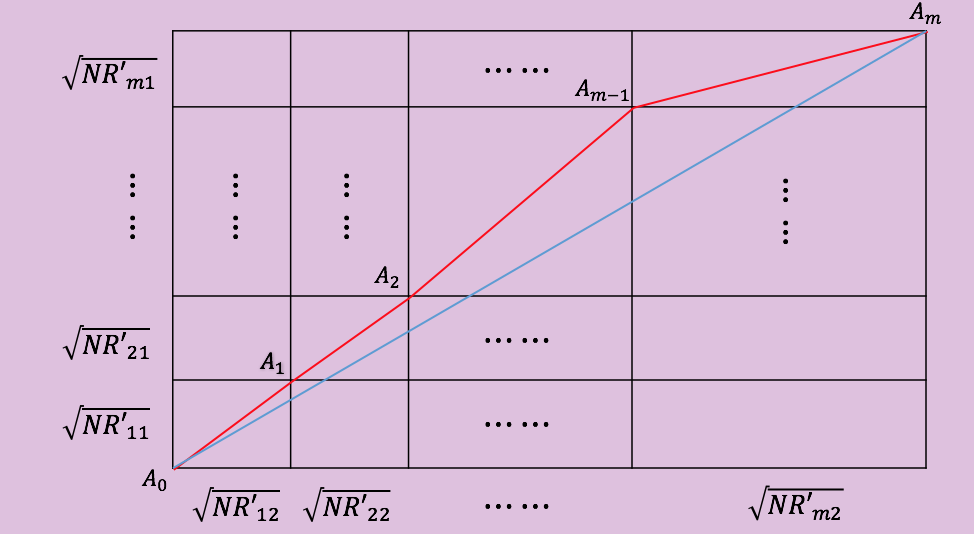
\includegraphics[width = 0.6\textwidth]{../common/m1.png}
   		 	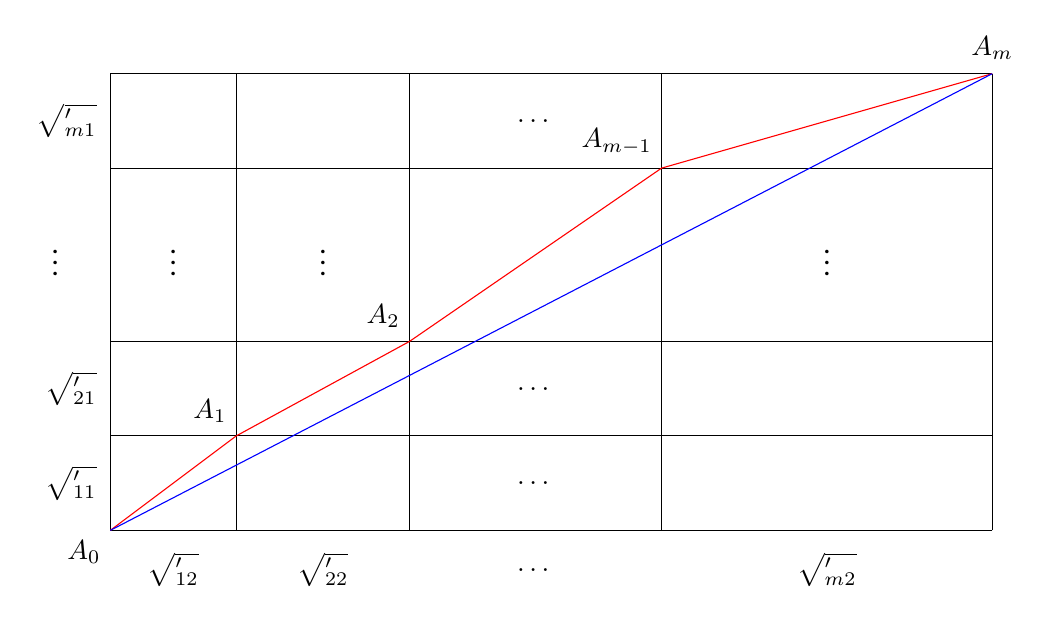
\begin{tikzpicture}
\pgfmathsetmacro{\HEIGHT}{1.2}
\pgfmathsetmacro{\HDOT}{2.2}
\pgfmathsetmacro{\WDOT}{3.2}
\pgfmathsetmacro{\WOne}{1.6}
\pgfmathsetmacro{\WTwo}{2.2}
\pgfmathsetmacro{\WN}{4.2}

\pgfmathsetmacro{\LEN}{\WOne + \WTwo + \WN + \WDOT}
\pgfmathsetmacro{\TH}{3*\HEIGHT+ \HDOT}

\tikzset{
  t/.style={draw, on grid, align=center, minimum height=1ex},
  coord/.style={coordinate, on grid, node distance=6mm and 25mm},
  between/.style args={#1 and #2}{
         at = ($(#1)!0.5!(#2)$)
    }
}

\draw [name path=h1] (0, 0) -- (\LEN, 0);
\draw [name path=h2] (0, \HEIGHT) -- (\LEN, \HEIGHT);
\draw [name path=h3] (0, 2*\HEIGHT) -- (\LEN, 2*\HEIGHT);
\draw [name path=h4] (0, 2*\HEIGHT + \HDOT) -- (\LEN, 2*\HEIGHT + \HDOT);
\draw [name path=h5] (0, 3*\HEIGHT + \HDOT) -- (\LEN, 3*\HEIGHT + \HDOT);

\draw[name path=v1] (0, 0) -- (0, \TH);
\draw[name path=v2] (\WOne, 0) -- (\WOne, \TH);
\draw[name path=v3] (\WOne + \WTwo, 0) -- (\WOne + \WTwo, \TH);
\draw[name path=v4] (\WOne + \WTwo + \WDOT, 0) -- (\WOne + \WTwo + \WDOT, \TH);
\draw[name path=v5] (\WOne + \WTwo + \WDOT + \WN, 0) -- (\WOne + \WTwo + \WDOT + \WN, \TH);

\path [name intersections={of=h1 and v1,by=A0}];
\path [name intersections={of=h2 and v2,by=A1}];
\path [name intersections={of=h3 and v3,by=A2}];
\path [name intersections={of=h4 and v4,by=Am1}];
\path [name intersections={of=h5 and v5,by=Am}];

\draw [red] (A0) -- (A1) -- (A2) -- (Am1) -- (Am);
\draw [blue] (A0) -- (Am);

\node [below=0.01 of A0, anchor=north east] {$A_0$};
\node [above=0.05 of A1, anchor=south east]{$A_1$};
\node [above=0.05 of A2, anchor=south east] {$A_2$};
\node [above=0.05 of Am1, anchor=south east] {$A_{m-1}$};
\node [above=0.05 of Am, anchor=south]{$A_m$};


\path [name intersections={of=h1 and v1,by=t00}];
\path [name intersections={of=h2 and v1,by=t01}];
\path [name intersections={of=h3 and v1,by=t02}];
\path [name intersections={of=h4 and v1,by=t03}];
\path [name intersections={of=h5 and v1,by=t04}];
\node [coord, between=t00 and t01] (x1){};
\node [coord, between=t01 and t02] (x2){};
\node [coord, between=t02 and t03] (x3){};
\node [coord, between=t03 and t04] (x4){};

\node [left=0.05 of x1.west] {$\sqrt{{\nr}'_{11}}$};
\node [left=0.05 of x2.west] {$\sqrt{{\nr}'_{21}}$};
\node [left=0.7 of x3.west, anchor=center] {$\vdots$};
\node [left=0.05 of x4.west] {$\sqrt{{\nr}'_{m1}}$};

\path [name intersections={of=h1 and v1,by=s00}];
\path [name intersections={of=h1 and v2,by=s01}];
\path [name intersections={of=h1 and v3,by=s02}];
\path [name intersections={of=h1 and v4,by=s03}];
\path [name intersections={of=h1 and v5,by=s04}];
\node [coord, between=s00 and s01] (y1){};
\node [coord, between=s01 and s02] (y2){};
\node [coord, between=s02 and s03] (y3){};
\node [coord, between=s03 and s04] (y4){};

\node [below=0.5 of y1.south, anchor=center] {$\sqrt{{\nr}'_{12}}$};
\node [below=0.5 of y2.south, anchor=center] {$\sqrt{{\nr}'_{22}}$};
\node [below=0.5 of y3.south, anchor=center] {$\dots$};
\node [below=0.5 of y4.south, anchor=center] {$\sqrt{{\nr}'_{m2}}$};

\node at (x1.east -| y3.north) {$\dots$};
\node at (x2.east -| y3.north) {$\dots$};
\node at (x4.east -| y3.north) {$\dots$};

\node at (y1.north |- x3.east) {$\vdots$};
\node at (y2.north |- x3.east) {$\vdots$};
\node at (y4.north |- x3.east) {$\vdots$};

\end{tikzpicture}

   		 	\caption{Proof by shortest distance\label{fig:path}}
   		 \end{figure}
   As shown in Figure~\ref{fig:path}, we construct a grid whose length and width are divided into $m$ segments,  the $i$-th segment of which has length $\sqrt{\nr'_{i1}}$ and $\sqrt{\nr'_{i2}}$ respectively. 
   
   	Then, $S_1^{'2}+S_2^{'2}=A_0A_m^2$, that is, equals to the square of the blue segment's length. In the meanwhile, 
   	 $$S_1^2 = (\sum_{i=1}^m \sqrt{\nr_{i1}})^2 > (\sum_{i=1}^m \sqrt{\nr'_{i1}+\nr'_{i2}})^2 = (\sum_{i=1}^m A_{i-1}A_i)^2$$,
   	 which equals to the sum of squares of all red segments. Since the shortest distance between two points is a line-segment, it holds that $S_1^2 >S_1^{'2}+S_2^{'2}$.
   	 
   	 For the cases where $k>2$ DApps are split, 	we can regard it as successive splits and iteratively use the result on $k=2$. 
   	 
   	 So the property is proved.
   	 
\end{proof}

\subsection{Proof of Corollary~\ref{c1}}
\label{subsection:proof3}
\begin{proof}
	For any voter that is bought over by $d_1$'s developer, before splitting, we can regard the voter as a normal voter who values all DApps with weight vector $(1,0,0,...,0)$, as he gives his all voting capacity to $d_1$. Suppose now $d_1$ is split into $k$ DApps and the bough-over voter's contributory values to the $k$ DApps are $\nr_{t1},...,\nr_{tk}$, whose sum is fixed. According to the condition that the equality holds for Cauthy's inequality in the proof of Property~\ref{p1}, the voter can be regard as a normal voter who values all DApps with weight vector $(\sqrt{\nr_{t1}}/C,\sqrt{\nr_{t2}}/C,...,\sqrt{\nr_{tk}}/C,0,0,...,0)$, where $C=\sum_{j=1}^k \sqrt{\nr_{tj}}$. That is, the voter values the split DApps with weights according to kind of proportion and values all other DApps with 0 weights.~\footnote{Note that scaling all weights by a constant does not effect the results, since the total contributory value of the voter only depends on the proportions of weights to total weights}. Since
		$$\sum_{j=1}^k \sqrt{\nr_{tj}}/C =1$$
	so the case in this corollary can be reduced to the case about normal voters(Property~\ref{p2}). So the corollary is proved.
\end{proof}

\subsection{Proof of Property~\ref{p3}}
\begin{proof}
	We first consider the case that a voter splits his account into two sub-accounts. We fix the actions of other voters. Let $c$ to be the original account and $a,b$ to be the split sun-accounts, $S,S'$ to be the ranking score of the DApp that the voter plans to vote before and after splitting respectively, $U,U'$ to be the final reward of the developer of the DApp that the voter plans to vote before and after splitting respectively. By definition, we have 
	$$S= \sqrt{\nr_c}+O,~~S'=\sqrt{\nr_a}+\sqrt{\nr_b}+O$$,
	where $O$ is the sum of contributory values by other voters, which is fixed. 
	
	By ~\ref{eq:sqrt_nr} it holds that $S < S'$. That is, the rank of the DApp does not increase. 
	
	In the meanwhile, by definition, 
	$$U = \frac{S}{S+P}\lambda M,~~U' = \frac{S'}{S'+P} \lambda M$$,
	where $P$ is the sum of squares of other DApp's ranking score, which is fixed. 
	
	Since $S < S'$ it holds that $U \leq U'$. That is the developer's final reward does not increase.
	
	For the cases where $k>2$ sub-accounts are split, we can regard it as successive splits and iteratively use the result on $k=2$. 
	
\end{proof}
\section{Registro de cambios}
\subsection{2019.4.8 registro de cambios}
\begin{itemize}
	\item Se reemplaza la función de NR a capacities (\ref{eq:capacity}) mediante $f(\mathcal{C}(a_i))=\mathcal{C}(a_i)$
	\item Se reemplaza el cálculo del factor de participación $\lambda$ (\ref{eq:participation}) mediante $\min\{\frac{0.008}{1-r},1\}$, donde $r=\frac{\nr_p}{\nr_s}$
	\item Se corrigen errores de tipeo.
\end{itemize}
\end{appendices}

\end{document}
